%%%%%%%
% Ch5 %
%%%%%%%

\chapter{Hacheurs à un quadrant - alimentations à découpage}	
	Pour une conversion DC/DC à un seul quadrant, des montages plus simples s'imposent. Le premier domaine d'application est celui des équipements électroniques qui incluent le plus souvent des \textbf{isolations galvaniques} pour la sécurité d'utilisation. Lorsque l'interrupteur du convertisseur DC/DC fonctionne en tout (état fermé, quasi-court-circuit) ou en rien (état ouvert, circuit quasi ouvert), on parle d'\textbf{alimentation à découpage} (switching mode power supply, SMPS) par opposition aux \textbf{alimentations linéaires}. 
	
	\section{Alimentations linéaires versus alimentations à découpage}
		\begin{wrapfigure}[12]{l}{5.5cm}
		\vspace{-5mm}
		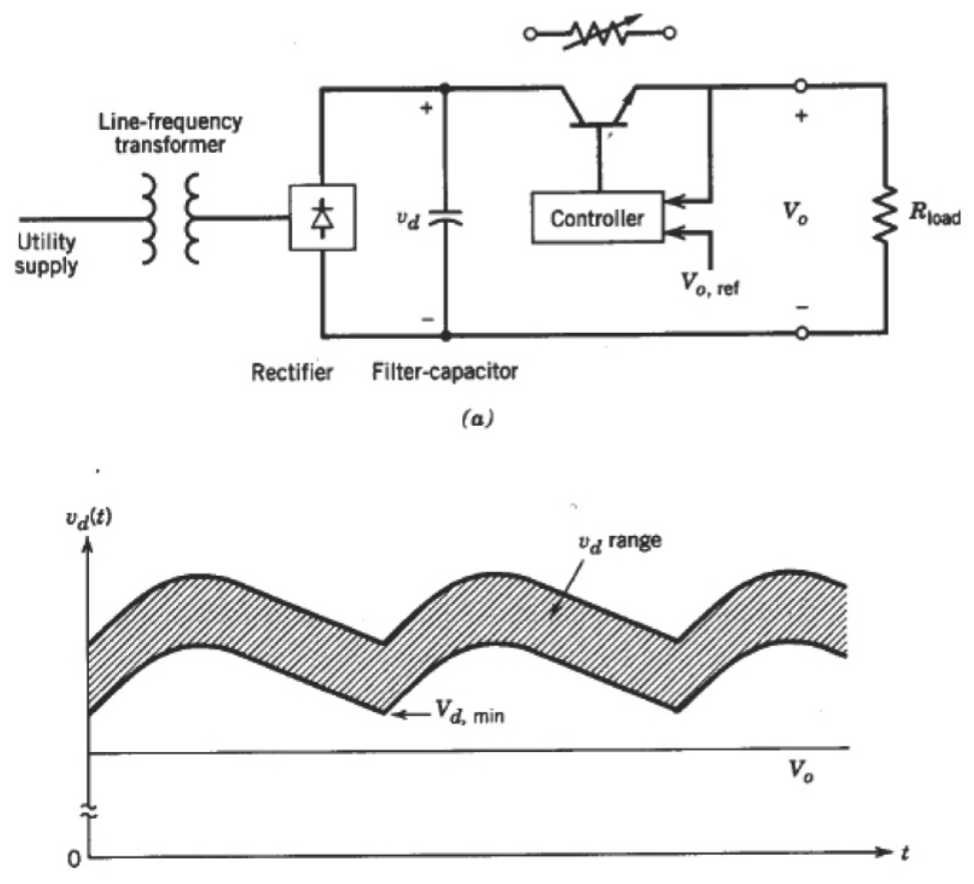
\includegraphics[scale=0.3]{ch5/1}
		\captionof{figure}{}
		\end{wrapfigure}
		Ci-contre se trouve un montage d'une alimentation linéaire. Le premier étage comprend un transformateur assurant aussi l'isolation galvanique entre AC et DC. Vient ensuite un redresseur à diode suivi d'un condensateur pour lisser la tension. À ce stade, $v_d(t)$ est toujours quelque peu ondulée (harmoniques multiples de 100Hz en cas de redressement monophasé) et sa tension moyenne varie selon la tension du réseau et de la charge. Avec le transfo, on fait en sorte d'avoir $V_d$ légèrement supérieur à $V_o$ souhaitée. C'est au transistor qui fonctionne dans sa région linéaire et se comporte comme une résistance commandable de niveler la tension vers le bas (pertes importantes). \\
		
		Les SMPS ont un meilleur rendement, sont plus compacts et moins chers. Le découpage se fait à une fréquence beaucoup plus grande que celle du réseau (kHz) $\Rightarrow$ taille considérablement réduite pour les composants magnétiques et condensateurs. Par contre, la commande est plus difficile et le découpage entraîne une déformation des tensions et courants AC et DC. 
		
\section{Topologie de base des hacheurs à un quadrant (buck, boost, buck-boost)}
	Les 3 hacheurs de base sont :
	\begin{itemize}
		\item[•] \textbf{hacheur buck} (hacheur dévolteur, série, step-down chopper, ...) 
		\item[•] \textbf{hacheur boost} (hacheur survolteur, parallèle, step-up, ...)
		\item[•] \textbf{hacheur buck-boost} (hacheur dévolteur-survolteur, ...)
	\end{itemize}
	\ \\
	
	On s'intéressera à des charges R avec une capacité en sortie pour lisser la tension. Ainsi chaque montage comprend un interrupteur T, une diode de roue libre D, une inductance L et un condensateur C. On observera une tension aux bornes de l'inductance $v_L(t)$ constante par morceau et $i_L(t)$ en dents de scie. Pour les buck et boost, on observe quasi les mêmes formes d'onde en présence de l'induit d'une mcc (RLE) en sortie (fonctionnement moteur) ou en entrée (fonctionnement dynamo). Pour ces machines, l'inductance de l'induit sera suffisante pour lisser le courant. 
	
	\subsection{Hacheur buck}	
	
		\begin{wrapfigure}[6]{l}{5.5cm}
		\vspace{-5mm}
		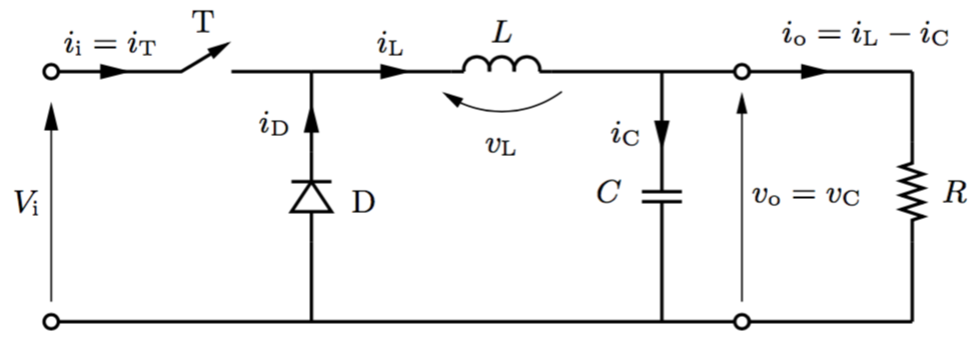
\includegraphics[scale=0.3]{ch5/2}
		\captionof{figure}{}
		\end{wrapfigure}	
		Ci-contre, le montage buck avec filtre LC et charge R avec $V_o < V_i$, avec $v_i= V_i$ supposé parfaitement lisse. Le courant $i_1$ circule dans T est non lisse.  
		
		\ \\\\
		 		
		\begin{wrapfigure}[6]{r}{4.5cm}
		\vspace{-5mm}
		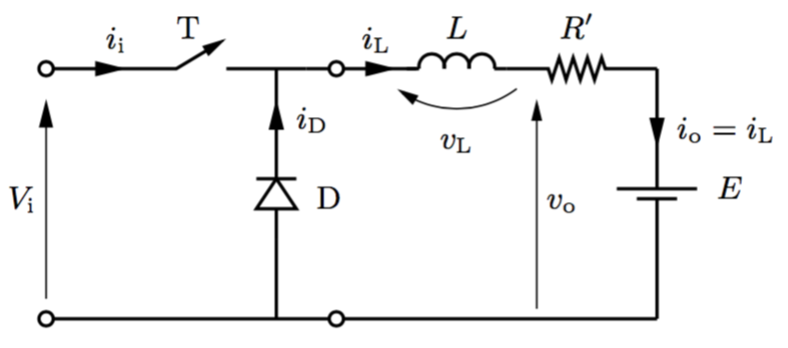
\includegraphics[scale=0.3]{ch5/3}
		\captionof{figure}{}
		\end{wrapfigure}	
		Ci-contre le montage équivalent avec un montage RLE. Avec certaines hypothèses, les formes d'onde, notamment $v_L$ et $i_L$ sont identiques à celles précédemment. On considérera par la suite le précédent montage avec une commande MLI. On démontrera que le filtre lisse mieux quand la fréquence de commutation $f_s$ de la MLI est grande devant la coupure $f_c = 1/(2\pi\sqrt{LC})$. On peut donc 
		
		\begin{wrapfigure}[9]{l}{5.5cm}
		\vspace{-5mm}
		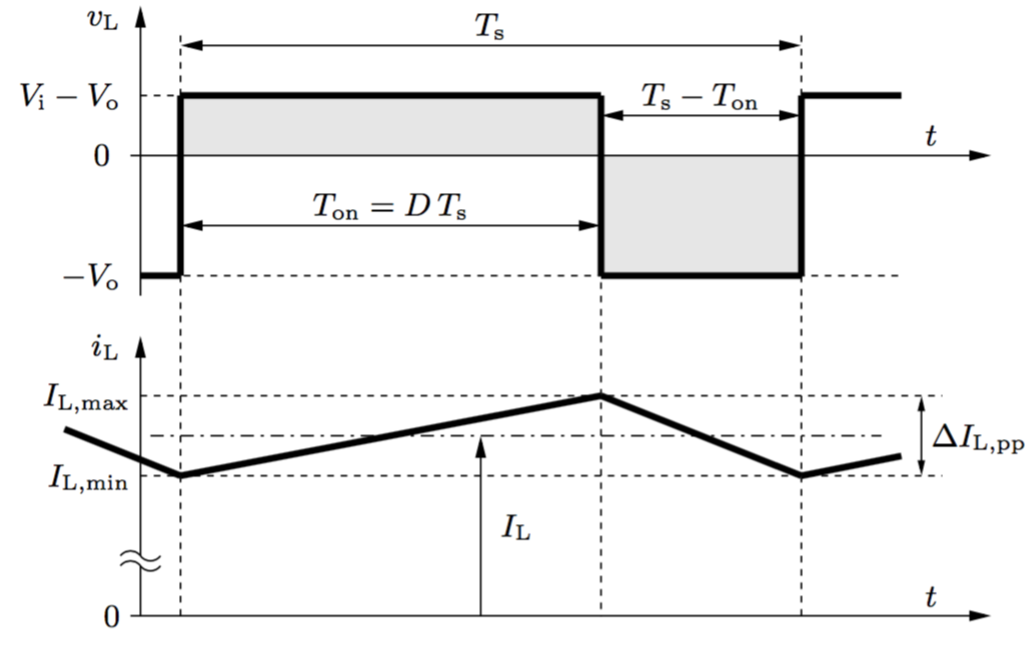
\includegraphics[scale=0.3]{ch5/4}
		\captionof{figure}{}
		\end{wrapfigure}	
		négliger l'ondulation de $v_o = v_C$, ainsi que les imperfections des composants. On utilisera de nouveau le rapport cyclique D (fermeture). À la fermeture de T, D est polarisé en inverse et $v_L = V_i - V_o>0$ avec un courant $i_L$ qui y augmente avec une pente $di_L/dt = (V_i -V_o)/L$.  
		
		\ \\Interrupteur ouvert, $i_L$ continue à circuler dans D et $v_L = -V_o<0$ avec $i_L$  qui diminue avec une pente $-V_o/L$. En régime établi $I_C = 0$, le courant de sortie moyen est alors : 
		\begin{equation}
			I_o = I_L.
		\end{equation}
		On suppose pour l'instant que la conduction est ininterrompue et donc que $i_L$ varie en dents de scie. En régime établi, $V_L$ moyen est nulle, il vient :
		\begin{equation}
			DT_s(V_o-V_i) - (1-D)T_sV_o = 0 \qquad \Leftrightarrow \qquad V_o = DV_i
			\label{eq:5.2}
		\end{equation}
		montrant que $V_o$ est bien compris entre 0 et $V_i$. Notons qu'on retrouve la même relation que dans le hacheur 2 quadrants demi-pont, mais dans le cas du buck n'est valable qu'en conduction ininterrompue. En considérant des composants idéaux et les tensions et courants parfaitement lisses, on trouve via le bilan de puissance le rapport $I_o/I_i$ :
		\begin{equation}
			V_iI_i = V_oI_o \qquad \Rightarrow \qquad \frac{I_o}{I_i}=\frac{1}{D}.
		\end{equation}		 
		Puisque $v_L=  -V_o$ durant $(1-D)T_s$, on a :
		\begin{equation}
			\Delta I_{L,pp} = I_{L,max}-I_{L,min} = (1-D)\frac{1}{f_sL}V_o = (1-D)D\frac{1}{f_sL}V_i
			\label{eq:5.4}
		\end{equation}
		
		\subsubsection{Ondulation de la tension de sortie}
			\begin{wrapfigure}[8]{l}{6cm}
			\vspace{-5mm}
			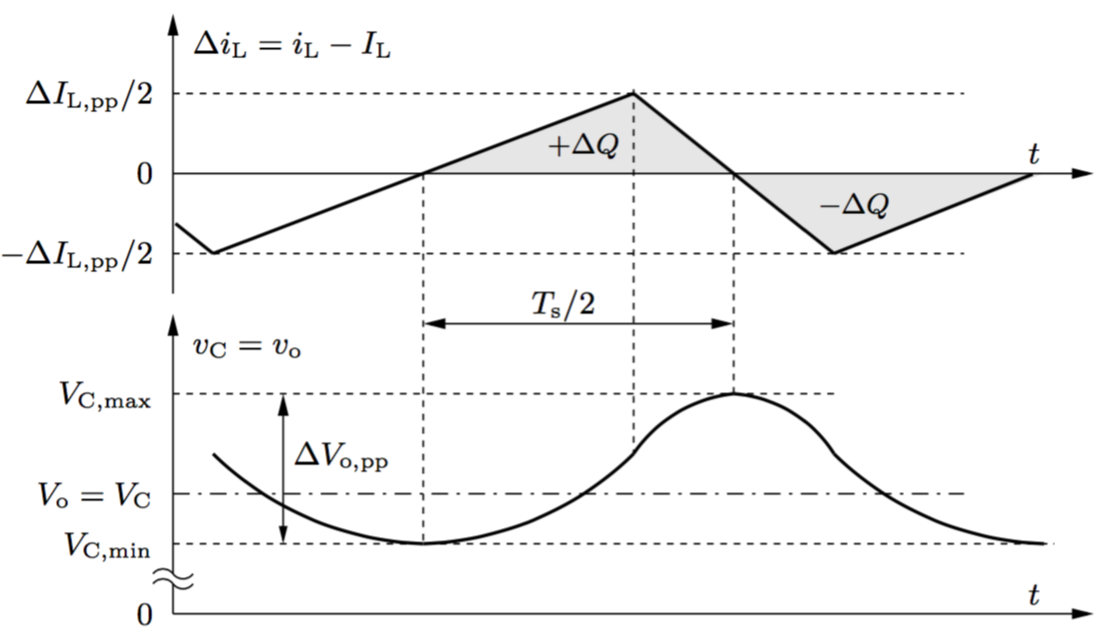
\includegraphics[scale=0.3]{ch5/5}
			\captionof{figure}{}
			\end{wrapfigure}	
			Le courant qui circule dans le condensateur est : 
			\begin{equation}
				i_C = i_L - \underbrace{i_o}_{\approx I_o = I_L}
			\end{equation}
			où on néglige l'ondulation de $i_o$ devant celle de $i_L$. $i_C$ est alors égal à la déformation de $i_L$ :
			\begin{equation}
				i_C = \Delta i_L = i_L -I_L.
			\end{equation}
			Il y correspond une variation de la charge du condensateur $q = \int i_C(t) \, dt$, et donc de $v_o = v_c = q/C$, respectivement autour de la charge moyenne $Q$ et la tension moyenne $V_o = V_c = Q/C$. Durant une alternance positive de $i_C$, $v_o$ monte à partir de $V_{C,min}$ pour atteindre $V_{C,max}$ à la fin de cette alternance; inversement pour l'alternance négative. La charge $\Delta Q$ retirée ou apportée est l'aire : 
			\begin{equation}
				\Delta Q = \frac{1}{2}\frac{T_s}{2}\frac{\Delta I_{L,pp}}{2} = \frac{1}{8f_s}\Delta I_{L,pp} \qquad \Rightarrow \qquad \Delta V_{o,pp} = \frac{\Delta Q}{C} = \frac{1}{8f_sC}\Delta I_{L,pp}.
			\end{equation}
			Avec \eqref{eq:5.4} et $f_c = 1/2\pi \sqrt{LC}$, l'ondulation relative donne : 
			\begin{equation}
				\frac{\Delta V_{o,pp}}{V_o} = \frac{1}{8}\frac{1}{f_s^2LC}(1-D) = \frac{\pi ^2}{2}\left(\frac{f_c}{f_s} \right)(1-D). 
			\end{equation}
			Pour un D donné, pour diminuer l'ondulation, on peut augmenter $f_s$ ou le produit LC au détriment de pertes de commutation plus importantes et/ou l'encombrement, poids et prix du convertisseur. 
			
		\subsubsection{Lien entre conduction ininterrompue et interrompue}
			\begin{wrapfigure}[5]{r}{6.5cm}
			\vspace{-5mm}
			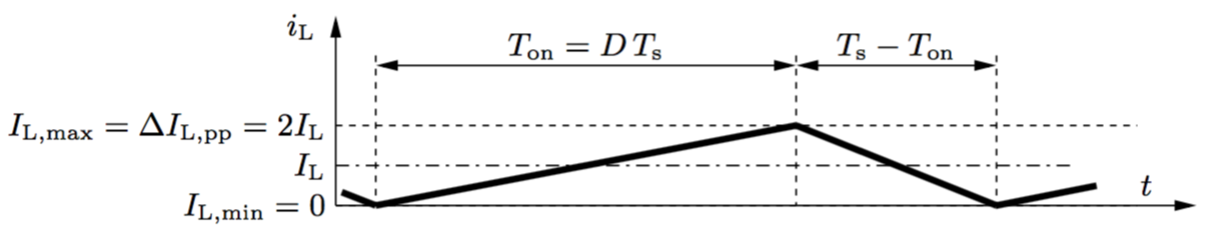
\includegraphics[scale=0.3]{ch5/6}
			\captionof{figure}{}
			\end{wrapfigure}	
			On remarque que R n'intervient pas dans les équations du cas ininterrompu, la capacité C oui. Pour $V_i, D$ et $f_s L$ fixés, l'augmentation de R cause la diminution de $I_L = I_o = V_o/R$ et de $I_{L,min}=I_L - \Delta I_{L,pp}/2$. Pour une certaine valeur de R, on atteint la limite entre conductions ininterrompue et interrompue : $I_{L,min}=0$. Dans ce cas limite, on a :
			\begin{equation}
				I_{o,lim} = I_{L,lim} = \Delta I_{L,pp}/2 = (1-D)\frac{1}{2f_sL}V_o = (1-D)D\frac{1}{2f_sL}V_i.
			\end{equation}
			Introduisons une valeur de référence de courant moyen pour la suite :
			\begin{equation}
				I_{o,ref} = \frac{1}{8f_sL}V_i \qquad \Rightarrow \qquad I_{o,lim} = 4(1-D)DI_{o,ref}.
			\end{equation}
			
		\subsubsection{Conduction interrompue}
			\begin{wrapfigure}[7]{l}{6.5cm}
			\vspace{-5mm}
			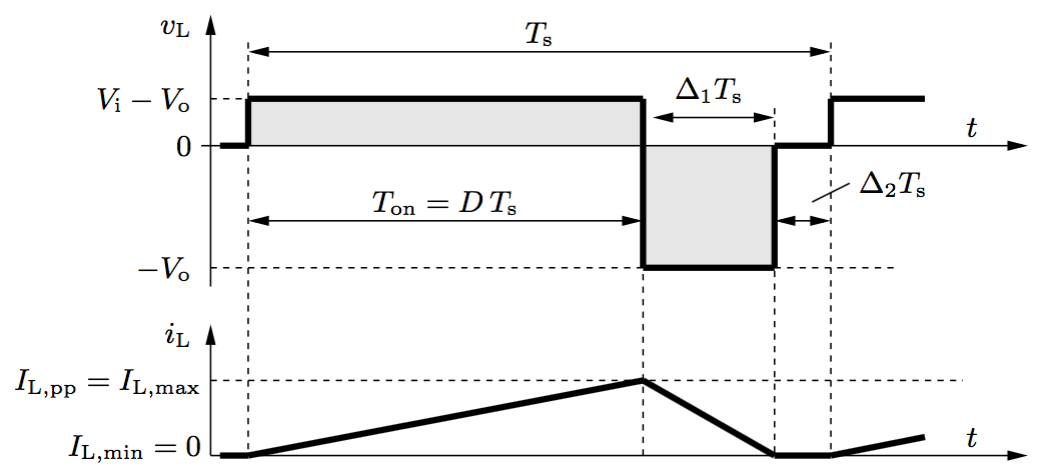
\includegraphics[scale=0.3]{ch5/7}
			\captionof{figure}{}
			\end{wrapfigure}	
			Dans ce cas $i_L(t)$ s'annule tout un intervalle à la fin de chaque cycle de commutation (avant refermeture) et $v_L(t)$ y est nul également. \eqref{eq:5.2} n'est alors plus valable et $V_o$ dépend également de $I_o$. Le cycle de commutation se divise en 3 intervalles :
			\begin{equation}
				D + \Delta _1 + \Delta _2 = 1 \qquad avec \qquad 0<\Delta < 1-D.
			\end{equation}
			
			En régime établi, $V_L = 0$ et donc :
			\begin{equation}
				DT_s (V_i - V_o) - \Delta _1 T_s V_o = 0 \qquad \Leftrightarrow \qquad \frac{V_o}{V_i} = \frac{D}{D+\Delta _1} > D. 
			\end{equation}
			
			On voit que $V_o$ est plus grand que dans le cas ininterrompu avec $V_i$ et $D$ fixés. Le courant de sortie moyen sera :
			\begin{equation}
				I_o = I_L = I_{L,max}\frac{D+\Delta _1}{2}\qquad avec \qquad I_{L,max} = D\frac{1}{f_sL}(V_i-V_o).
			\end{equation}
			
			\begin{wrapfigure}[8]{l}{6cm}
			\vspace{-5mm}
			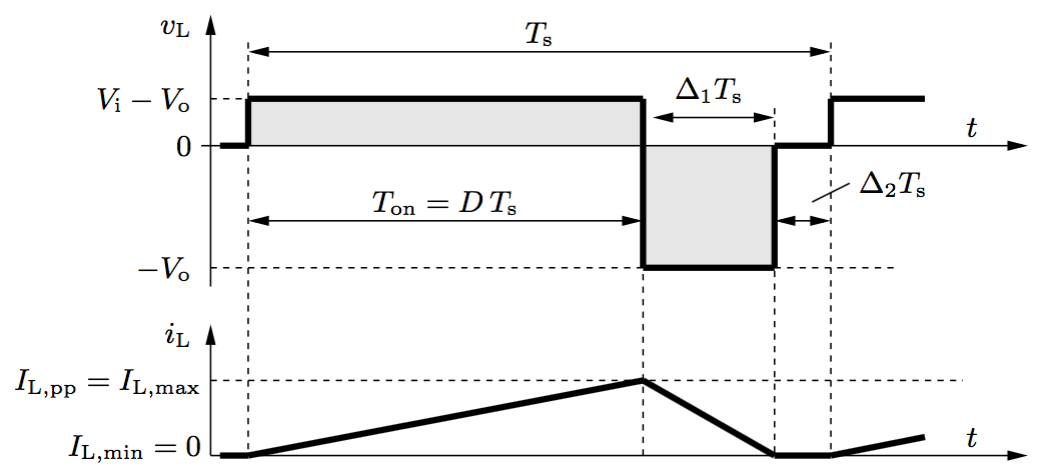
\includegraphics[scale=0.3]{ch5/7}
			\captionof{figure}{}
			\end{wrapfigure}	
			En combinant les 2 précédentes équations et $I_{o,ref}$, on obtient :
			\begin{equation}
				\frac{V_o}{V_i} = \frac{D^2}{D^2+\frac{1}{4}I_o/I_{o,ref}}.
			\end{equation}
			Ci-contre est montrée la dépendance en $I_o/I_{o,ref}$ en considérant la zone interrompue et ininterrompue. Dans la seconde zone, $\frac{V_o}{V_i} = D$, $I_o$ n'a aucune influence. Notons que le fonctionnement à résistance de charge R  correspond à une droite passant par l'origine sur notre figure ci-contre :
			\begin{equation}
				\frac{V_o/V_i}{I_o/I_{o,ref}} = \frac{V_o}{I_o}\frac{I_{o,ref}}{V_i} = \frac{R}{8 f_s L}.
			\end{equation}
			
			Pour $R=\infty$ (absence de charge), $V_o = V_i$ pour le régime établi. En effet, aucun chemin de décharge n'est disponible pour le condensateur qui ne peut pas être chargé par $i_L\leq  0$ pendant le transitoire préalable au fonctionnement à vide. 
			
	\subsection{Hacheur boost}
		\begin{center}
		\begin{minipage}{0.45\textwidth}
			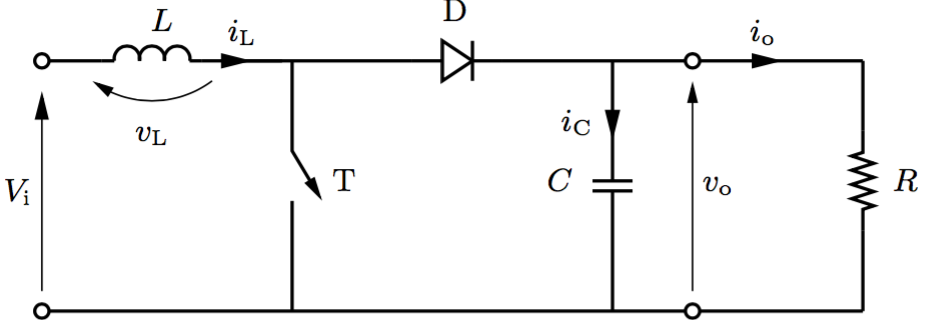
\includegraphics[scale=0.42]{ch5/9}
			\captionof{figure}{}
		\end{minipage}
		\begin{minipage}{0.45\textwidth}
			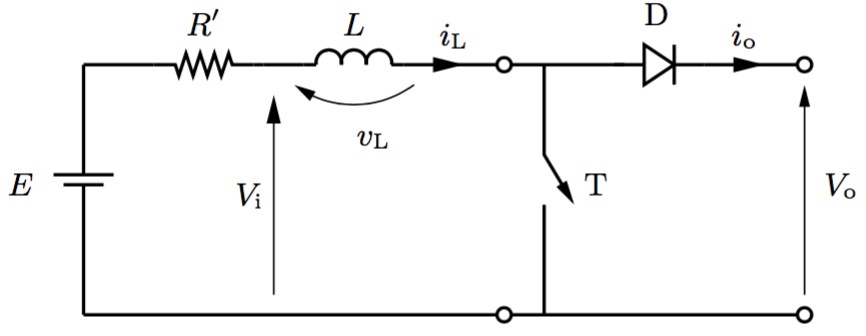
\includegraphics[scale=0.41]{ch5/10}
			\captionof{figure}{}
		\end{minipage}
		\end{center}
		
		\begin{wrapfigure}[9]{r}{6cm}
		\vspace{-5mm}
		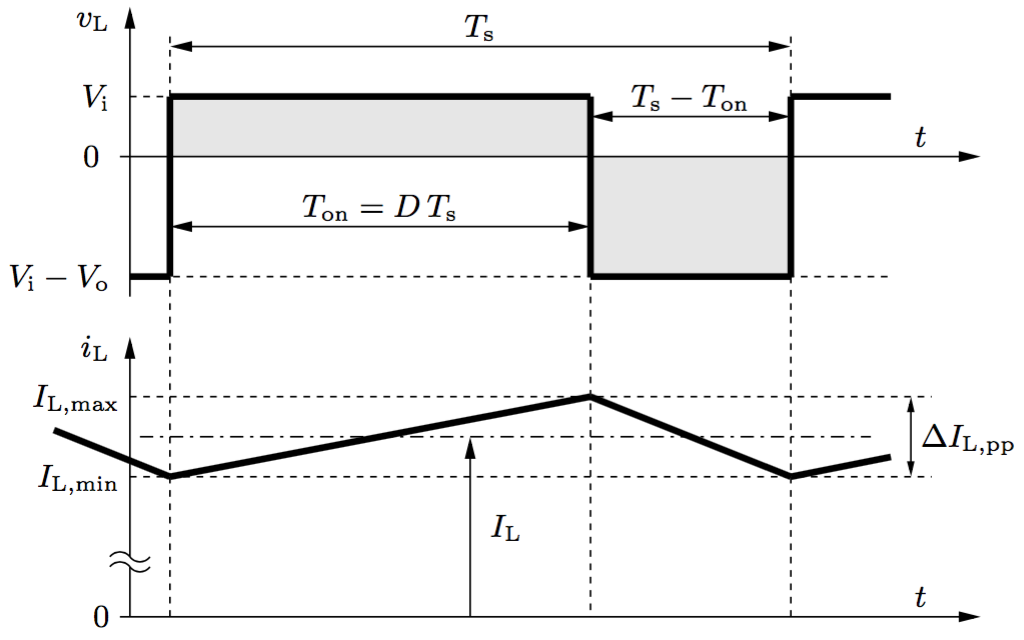
\includegraphics[scale=0.3]{ch5/11}
		\captionof{figure}{}
		\end{wrapfigure}	
		Le montage ci-dessus (gauche) est issu du réarrangement du montage buck, avec lissage de la tension de sortie par un condensateur. La figure de droite représente le cas comparatif avec une charge RLE en entrée et une source de tension en sortie (induit mcc fonctionnant en dynamo). 
		
		\ \\ Comme précédemment, la commande MLI donne lieu à $i_L(t)$ en dents de scie dans le cas ininterrompu. Lorsque l'interrupteur est fermé, $v_D = -V_o$ et $v_L(t) = V_i >0$ avec $i_L(t)$ qui augmente avec une pente $V_i/L$. Lorsque l'interrupteur est ouvert, $v_L(t) = V_i - V_o < 0$ et $i_L$ circulant dans la diode de roue libre diminue avec une pente $(V_i - V_o) /L$. La tension moyenne aux bornes de l'inductance étant nulle :
		\begin{equation}
			DT_s V_i + (1-D)T_s (V-i-V_o) = 0 \qquad \Leftrightarrow \qquad V_o = \frac{1}{1-D}V_i. 
		\end{equation}
		On voit que $V_o \geq V_i$ en accord avec les dénominations de ce hacheur. 
		
		\begin{wrapfigure}[5]{l}{3.5cm}
		\vspace{-5mm}
		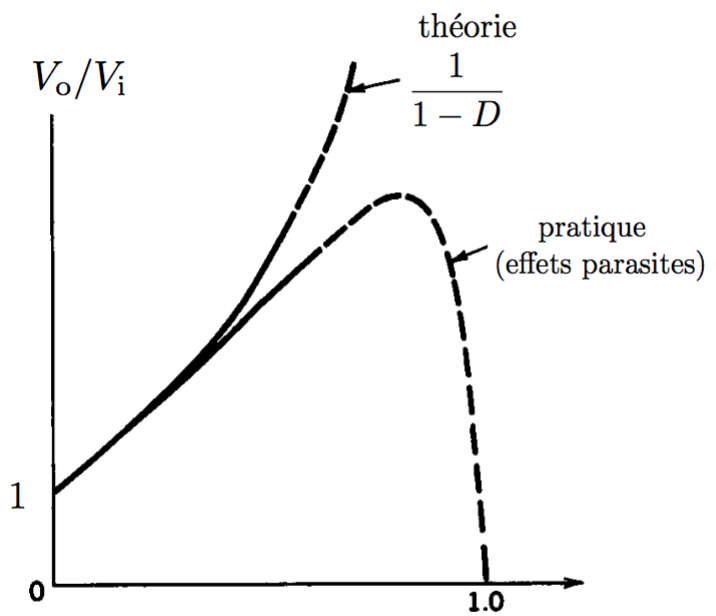
\includegraphics[scale=0.25]{ch5/12}
		\captionof{figure}{}
		\end{wrapfigure}	
		La figure ci-contre montre la caractéristique théorique et on voit que la théorie $\rightarrow \infty$ pour D $\rightarrow 1$ alors que la pratique est déformée suite aux effets parasites des composants réels (tension résiduelle de l'interrupteur et diode, résistance bobine/condensateur, ...).   \\\\
		
	\subsection{Hacheur buck-boost}
		\begin{wrapfigure}[3]{r}{5.1cm}
		\vspace{-16mm}
		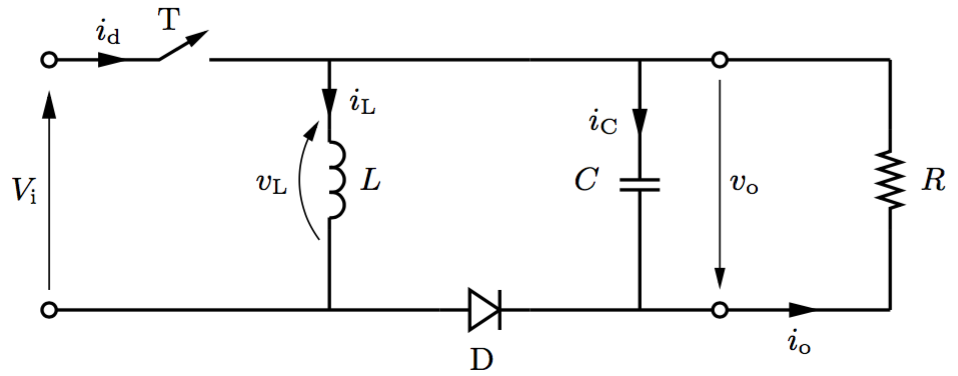
\includegraphics[scale=0.3]{ch5/13}
		\captionof{figure}{}
		\end{wrapfigure}	
		Encore une autre disposition des composants donne le montage ci-contre pour le convertisseur buck-boost, avec condensateur de lissage et une charge R. 
		
		\ \\
		\begin{wrapfigure}[8]{l}{4.5cm}
		\vspace{-5mm}
		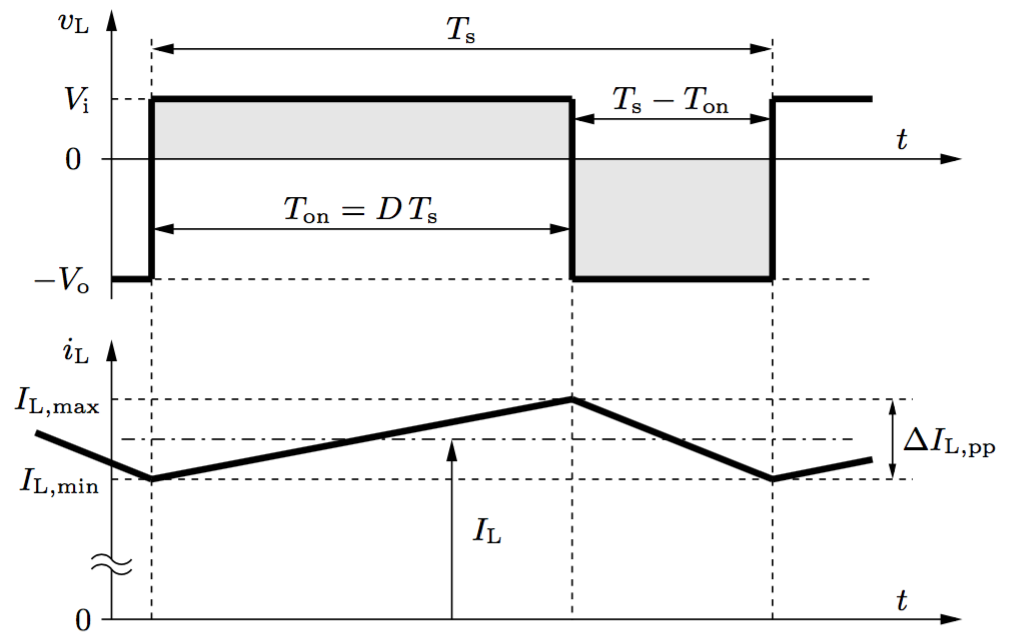
\includegraphics[scale=0.25]{ch5/14}
		\captionof{figure}{}
		\end{wrapfigure}	
		$i_L(t)$ varie de nouveau en dents de scie en ininterrompu. Lorsque l'interrupteur est fermé, $v_L(t) = V_i$ et $i_L$ monte. Lorsque T est ouvert, $v_L = V_o$ parce que cette fois $V_o$ est prise dans le sens inverse (vers le bas). De nouveau, pour $V_L = 0$ en ininterrompu : 
		\begin{equation}
			DT_s V_i - (1-D)T_s V_o = 0 \qquad \Leftrightarrow \qquad V_o = \frac{D}{1-D}V_i.
		\end{equation}
		On peut donc avoir $V_o \leq V_i$ ou $V_o \geq V_i$. Pour $D = 0.5$, $V_o =V_i.$ \\ 
		
		\begin{wrapfigure}[6]{r}{4.5cm}
		\vspace{-5mm}
		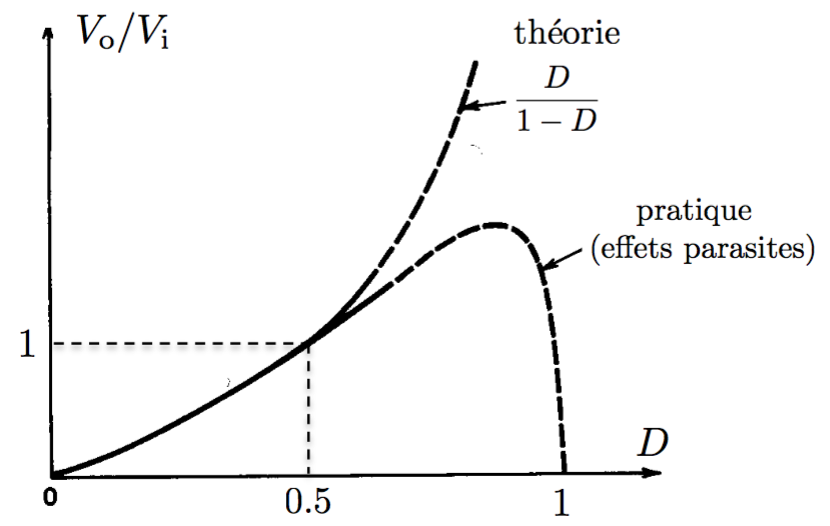
\includegraphics[scale=0.3]{ch5/15}
		\captionof{figure}{}
		\end{wrapfigure}	
		Notons que l'inversion de $V_o$ peut être un avantage. Ci-contre se trouve la caractéristique. Remarquons finalement que le rapport $D/(1-D)$ peut s'obtenir via la mise en cascade d'un buck et d'un boost aux dépens d'un coût plus important et un rendement moindre du fait du doublement du nombre de composants. 
		
\section{Hacheurs avec isolation galvanique}
	\begin{wrapfigure}[7]{l}{6cm}
	\vspace{-5mm}
	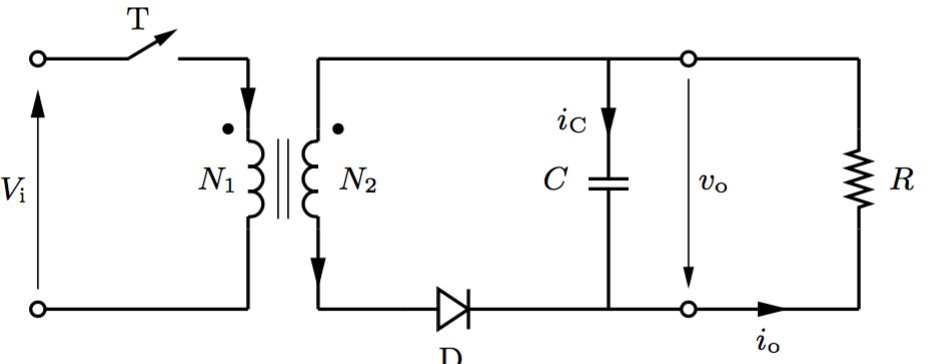
\includegraphics[scale=0.35]{ch5/16}
	\captionof{figure}{}
	\end{wrapfigure}	
	Les effets parasites deviennent important au plus l'écart des tensions devient trop importante. De plus, pour une puissance donnée $V_oI_o = V_iI_i$, si on fait abstraction des pertes, c'est la plus grande tension des deux qui détermine la capacité en tension $V_{T,max}$ pour T alors que c'est le plus grand courant pour la capacité en courant $I_{T,max}$. De ce fait, la capacité en puissance est d'autant moins bien utilisée que l'écart entre $V_o$ et $V_i$ et donc $I_o et I_i$ est grand. Dans ces cas-là, il convient d'incorporer un \textbf{transformateur} fonctionnant à la fréquence de commutation $f_s$. La figure ci-contre montre l'exemple du convertisseur \textbf{flyback} (buck-boost avec inductance remplacée par transfo). En conduction ininterrompue, les tensions sont liées :
	\begin{equation}
		V_o = \frac{D}{1-D}\frac{N_2}{N_1} V_i.
	\end{equation}
	
	 Il ne s'agit pas d'un transfo classique. De 1, il fonctionne à fréquence élevée, ce qui le rend compact. En conséquence, on a des noyaux massifs en ferrite au lieu de noyaux feuilletés en tôles magnétiques. De 2, il doit servir de tampon d'énergie tout comme l'inductance qu'il remplace. Ce stockage d'énergie est réalisé avec un noyau à entrefer, car la densité magnétique $\frac{1}{2}B^2/\mu$ de l'air ($\mu _0$) est plus grande que celle du fer ($\mu \gg$).
